%!TEX root = ../../super_main.tex

\section{Sensor Providers}
\label{sec:sensor_providers}

We have implemented a threaded abstraction over the different data sources that the system should utilize in order to gather context for the labels that will eventually be combined to form the output training data for the system. The abstraction is threaded because we want the Android application to be able to gather information from multiple sources concurrently. This is done in order to make sure that the gathered data is obtained temporally close to when the label for the data was obtained. 

\subsection{Napkin Mathematics}
\label{sub:napkin_mathematics}

As described in \secref{sec:availability_of_data_sources}, some data sources are continuous. We have experimented with the accelerometer sensor, which is an example of a continuous sensor, in a Nexus 5 smart phone and logged all values captured from the sensor for one minute. This gave us a dataset with a size of 142908 bytes. This experiment would then yield a data set of approximately 205 MB if it was run for a day. Running the same experiment for 30 days with 100 different devices would then approximately yield a data set of 617 GB assuming similar mobile devices with similar sensors. This quick napkin math was only for one sensor with 100 people and this could quickly escalate if more sensor or more people are added. 
\\\\
This could quickly become infeasible for both the users from whom the data is gathered and for the customers whom needs the data. These quantities of data might present a problem even on modern mobile platforms due to paid limited data plans and battery consumption, even in 2016. There might be different data needs, some customers might require very detailed data from many sensors from a few devices and others might require more sparse data from a few sensors from a lot of different devices. 

% Træls for bruge
% Træls for folk der kan bruge data

\subsection{Temporality}

% Det bliver hurtigt til meget data når man arbejder med continious data
% Vi bruger sample frequency til at lave mellemrum mellem samples i tid fordi det ikke er så brugbart at have 8gb data for et minuts målinger
% Vi vil gerne have flere measurements per sample så vi kan undgå upræcise målinger

We have come up with a solution to the concerns described in \secref{sub:napkin_mathematics}. We have decided to facilitate periodic data collection instead of continues readings of data in order to facilitate different data needs.

\begin{figure}[!htbp]
    \centering
    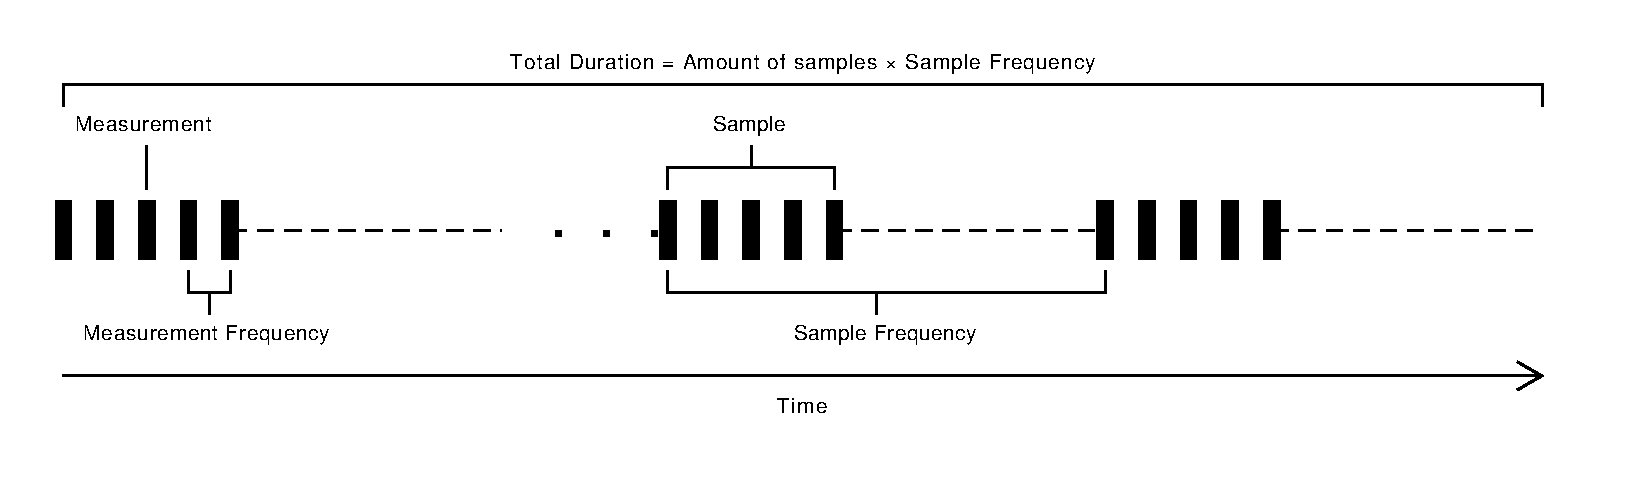
\includegraphics[width=\textwidth]{unsorted/sample_temporality}
    \caption{Overview of sample and measurement temporality.}
    \label{fig:sample_temporality}
\end{figure}

\subsection{Implementation}

The solution was to abstract data collection away in subclasses of a class called.. \todo{Write more}

% Future<T> Objects
% 

% \lstinputlisting[
%    style = java,
%    caption = {Property similarity on a component.},
%    label = {lst:attribute_difference},
%]{content/implementation/annotation/attribute_difference.java}